\subsection{Anforderungen}
Das Webinterface hat auf der einen Seite die Aufgabe die Kommunikation mit der
Kennzeichenerkennung und der Induktionmessung sicherzustellen und auf der
anderen Seite die Verwaltung und Darstellung der gewonnen Daten.

\subsection{Lokale Entwicklungsumgebung mit Laragon}
Für die Programmierung des Webinterfaces müssen zuerst einige Vorkehrungen
getroffen werden, dazu zählt zu einem die Installation von benötigter Software
und deren konfiguration.

\subsubsection{Benötigte Software}

\begin{itemize}
  \item \textbf{Laragon} (\url{https://laragon.org}) \\Beinhaltet mehrere
  Softwarepakete die für die Entwicklung notwendig sind.
  \begin{itemize}
    \item Apache HTTP Server
    \item MySQL
    \item PHP
  \end{itemize}
  \item \textbf{Composer} (\url{https://getcomposer.org}) \\ Paketmanager für
  PHP
  \item \textbf{Git} (\url{https://git-scm.com}) \\ Versionskontrolle
  \item \textbf{Visual Studio Code} (\url{https://code.visualstudio.com}) \\
  Quelltext-Editor
\end{itemize}

\subsubsection{Konfiguration von PHP}
Um PHP Befehle von der Kommandozeile auszuführen muss die Installation zuerst in
den Windows Path Variables hinzugefügt werden.

Dies erfolgt durch die \textbf{Advanced System Settings} $\blacktriangleright$
\textbf{Environment Variables} $\blacktriangleright$ \textbf{System Variables}.
Dort kann nun die Path Variable editiert werden und der Pfad hinzugefügt werden
in welchem die php.exe liegt.

\begin{figure}[H]
  \centering
  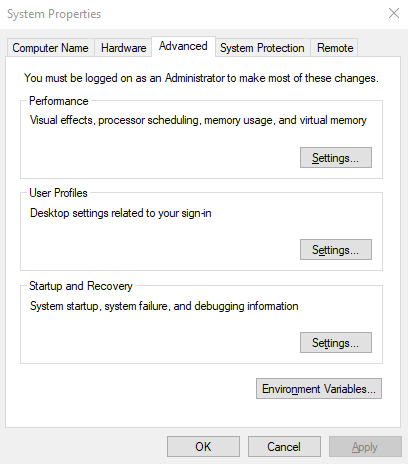
\includegraphics[width=0.6\linewidth]{advanced_system_settings.png}
  \caption{Advanced System Settings}
\end{figure}

\begin{figure}[H]
  \centering
  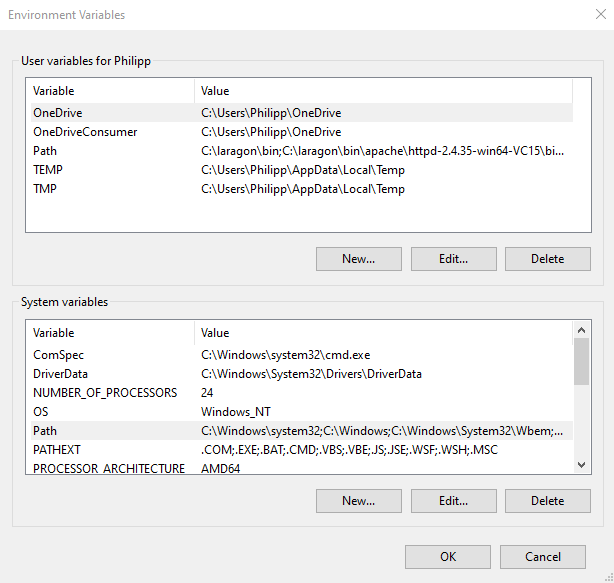
\includegraphics[width=0.6\linewidth]{system_variables.png}
  \caption{System Variables}
\end{figure}

\begin{figure}[H]
  \centering
  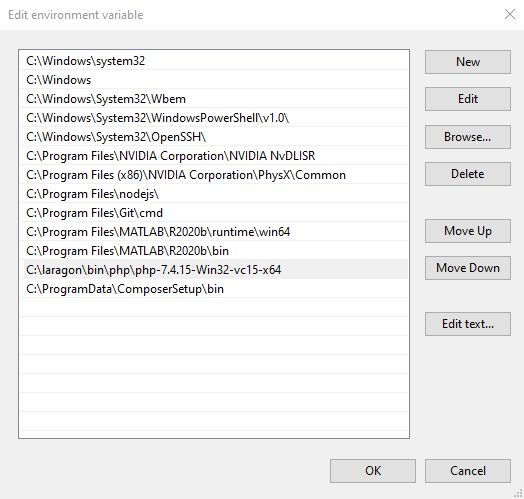
\includegraphics[width=0.6\linewidth]{environment_variable.png}
  \caption{Environment Variables}
\end{figure}

Die korrekte konfiguration kann durch die Kommandozeile geprüft werden, dort
muss das Befehl \textbf{php -v} ausgeführt werden. Dabei ist zu beachten, dass
nach dem hinzufügen der Path Variable die gewählte Kommandozeile neu gestartet
werden muss.

\begin{figure}[H]
  \centering
  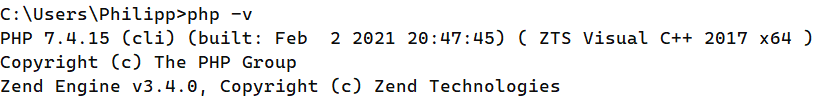
\includegraphics[width=1\linewidth]{php_version.png}
  \caption{PHP Version}
\end{figure}

Somit ist PHP korrekt konfiguriert.

\subsubsection{Installation von phpMyAdmin}
phpMyAdmin ist ein Tool, welches den Umgang mit MySQL Datenbanken mit einem
Webinterface erleichtert. Die aktuellste Version lässt sich von
\url{https://www.phpmyadmin.net/downloads} downloaden. Dieses Archiv muss
entpackt werden und ausgehend vom Laragon Root Verzeichnis in das Verzeichnis
\textbf{/etc/apps} kopiert werden. Um die Installation zu überprüfen muss der
Apache HTTP Server und der MySQL Server gestartet werden, nun sollte bei einer
korrekten Installation das Webinterface von phpMyAdmin unter
\url{http://localhost/phpmyadmin} erreichbar sein.

\begin{figure}[H]
  \centering
  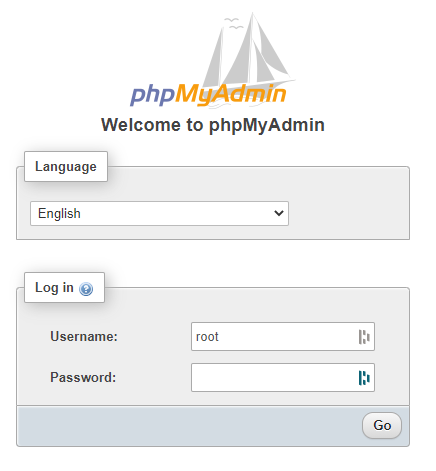
\includegraphics[width=0.5\linewidth]{phpmyadmin.png}
  \caption{phpMyAdmin Webinterface}
\end{figure}

Es ist nicht notwendig ein Passwort einzugeben, da Standardmäßig kein Passwort
gesetzt wird.

\subsection{Lokale Entwicklungsumgebung mit WSL und Docker}

\subsubsection{Benötigte Software}

\begin{itemize}
  \item \textbf{Docker} (\url{https://www.docker.com}) \\ Ermöglicht Isolation
  von Anwendungen mit Containervirtualisierung
  \item \textbf{WSL} (\url{https://docs.microsoft.com/en-us/windows/wsl}) \\
  Kompatibilitätsschicht für Linux Anwendungen unter Windows 10
  \item \textbf{Visual Studio Code} (\url{https://code.visualstudio.com}) \\
  Quelltext-Editor
\end{itemize}

\subsubsection{Installation von WSL}
Zuerst müssen einige Einstellungen in Windows getroffen werden um später eine
Linux Distribution herunterzuladen können. Diese Befehle können über die
Kommandozeile mit Administrativen Rechten ausgeführt werden.

\paragraph{1. Schritt: WSL Aktivieren}\mbox{}\\
\begin{lstlisting}[caption={WSL Feature Feature aktivierens}, captionpos=b]
  dism.exe /online /enable-feature
  /featurename:Microsoft-Windows-Subsystem-Linux /all /norestart
\end{lstlisting}

\paragraph{2. Schritt: Virtual Machine Aktivieren}\mbox{}\\
\begin{lstlisting}[caption={Virtual Machine Feature aktivieren}, captionpos=b]
  dism.exe /online /enable-feature
  /featurename:VirtualMachinePlatform /all /norestart
\end{lstlisting}

Nach diesem Schritt ist ein Neustart des Computers notwendig.

\paragraph{3. Schritt: Linux Kernel Update}\mbox{}\\
Nun muss ein Linux Kernel Update installiert werden, die aktuelle Version ist unter \url{https://aka.ms/wsl2kernel} zu finden.

\paragraph{4. Schritt: WSL 2}\mbox{}\\
Nach dem Neustart des Computers sollte es nun möglich sein WSL 2 als Version auszuwählen.
\begin{lstlisting}[caption={WSL 2 auswählen}, captionpos=b]
  wsl --set-default-version 2
\end{lstlisting}

\paragraph{5. Schritt: Linux Distribution herunterladen}\mbox{}\\
Zuletzt kann eine Linux Distribution aus dem Windows Store heruntergeladen werden, in diesem Fall Debian (\url{https://www.microsoft.com/de-de/p/debian}).

\subsubsection{Installation von Docker}
